%% Draft manuscript for Springer Nature / Neural Computing and Applications style.
%% Compile on Overleaf or locally with the official Springer Nature template files:
%% sn-jnl.cls, sn-mathphys-num.bst, and related files.
%% Suggested class option for NCA-like math/engineering manuscript:
\documentclass[pdflatex,sn-mathphys-num]{sn-jnl}

\usepackage{graphicx}
\usepackage{multirow}
\usepackage{amsmath,amssymb,amsfonts}
\usepackage{amsthm}
\usepackage{mathrsfs}
\usepackage[title]{appendix}
\usepackage{xcolor}
\usepackage{textcomp}
\usepackage{manyfoot}
\usepackage{booktabs}
\usepackage{algorithm}
\usepackage{algorithmicx}
\usepackage{algpseudocode}
\usepackage{listings}
\usepackage{bm}
% \jyear{2026}

% \theoremstyle{thmstyleone}
\newtheorem{theorem}{Theorem}
\newtheorem{proposition}[theorem]{Proposition}
% \theoremstyle{thmstyletwo}
\newtheorem{example}{Example}
\newtheorem{remark}{Remark}
% \theoremstyle{thmstylethree}
\newtheorem{definition}{Definition}

\newcommand{\R}{\mathbb{R}}
\newcommand{\N}{\mathbb{N}}
\newcommand{\calG}{\mathcal{G}}
\newcommand{\calN}{\mathcal{N}}
\newcommand{\calP}{\mathcal{P}}
\newcommand{\calR}{\mathcal{R}}
\newcommand{\calT}{\mathcal{T}}
\newcommand{\KNN}{\operatorname{KNN}}
\newcommand{\RNN}{\operatorname{RNN}}
\newcommand{\rdeg}{\operatorname{rdeg}}
\newcommand{\argmax}{\operatorname*{arg\,max}}

\graphicspath{{./}{figures/}{figures/2018/}{figures/generated/}}

\begin{document}

\title[Round-trip KNN graph clustering]{Round-trip closure on directed k-nearest-neighbor graphs for multiscale clustering}

\author*[1]{\fnm{Eraldo P.} \sur{Marinho}}\email{pereira.marinho@unesp.br}
\author[1]{\fnm{Caetano Mazzoni} \sur{Ranieri}}\email{cm.ranieri@unesp.br}
\author[1]{\fnm{Fabricio A.} \sur{Breve}}

\affil*[1]{\orgdiv{Department of Statistics, Applied Mathematics and Computing},
\orgname{S\~ao Paulo State University (UNESP), Institute of Geosciences and Exact Sciences},
\orgaddress{\street{Av. 24-A, 1515}, \city{Rio Claro}, \state{S\~ao Paulo}, \country{Brazil}}}

\abstract{
We introduce a graph-based clustering formulation based on recursive round-trip closure on directed $k$-nearest-neighbor graphs. The method is motivated by an earlier relational model in which an asymmetric relation $T\subseteq A\times B$ induces a reflective operator $R_T=T^{-1}\circ T$, and by a subsequent KNN-based model in which each nearest neighbor can reveal its reverse-neighbor set. In the present formulation, a data point first reaches one or more of its $K$ nearest neighbors, and each selected neighbor returns the set of data points that also selected it as one of their $K$ nearest neighbors. This forward-backward operation induces local popularity, leadership, and recursive expansion until saturation. Repeating the process across increasing values of $K$ produces a multiscale sequence of cluster layers, allowing cluster persistence, absorption, and merging to be analyzed through overlap transitions. The method is positioned as a nearest-neighbor graph clustering variant combining directed KNN topology, reverse-neighbor popularity, round-trip closure, saturation depth, and $K$-layer analysis. Preliminary synthetic results indicate that the generated layers are valid partitions, with no internal overlap among cluster memberships for each analyzed value of $K$.
}

\keywords{k-nearest-neighbor graph, graph-based clustering, reverse nearest neighbors, shared nearest neighbors, round-trip closure, multiscale clustering, saturation, cluster hierarchy}

\maketitle

\section{Introduction}\label{sec:introduction}

Nearest-neighbor relations are among the most fundamental structures used to represent finite datasets embedded in metric spaces. They occur naturally in pattern classification, nonparametric density estimation, graph construction, manifold learning, outlier detection, and clustering \citep{CoverHart1967,LoftsgaardenQuesenberry1965,Bentley1975,FriedmanBentleyFinkel1977,VonLuxburg2007}. In clustering, k-nearest-neighbor (KNN) relations have been explored through shared nearest neighbors, reciprocal nearest neighbors, mutual KNN graphs, reverse nearest-neighbor statistics, and density-based graph connectivity \citep{JarvisPatrick1973,ErtozSteinbachKumar2003,BritoChavezQuirozYukich1997,GowdaKrishna1978,ChowdhuryAmorim2018,XieLeeWangChenZhou2019}.

This paper develops a clustering formulation based on a recursive \emph{round-trip} operation in directed KNN graphs. Given a data point $x_i$, the forward step reaches one of its $K$ nearest neighbors, say $x_j\in\calN_K^+(x_i)$. The backward step then retrieves all data points that also selected $x_j$ as one of their $K$ nearest neighbors:
\begin{equation}
\calN_K^-(x_j)=\{x_\ell\in X: x_j\in\calN_K^+(x_\ell)\}.
\end{equation}
Thus, a neighbor is not used merely as a point in Euclidean space, but as an index to a reverse-neighborhood set. This operation can be recursively applied until no additional points are reached, producing a saturated closure.

The method has two historical sources. The first is a relational model of redundancy-based information transport, in which an asymmetric relation $T\subseteq A\times B$ induces a reflective composition $T^{-1}\circ T$. The second is a KNN-based clustering model, where a data point elects a locally popular neighbor by inspecting reverse-neighbor cardinalities. The present contribution is not the isolated use of KNN graphs, reverse nearest neighbors, or shared-neighbor similarity. Rather, it is the organization of these elements into a recursive closure process whose evolution across $K$ values defines a multiscale cluster-layer structure.

The main contributions are as follows:
\begin{enumerate}
    \item a formal round-trip operator on directed KNN graphs based on forward nearest-neighbor selection and backward reverse-neighbor retrieval;
    \item a popularity-based local leadership mechanism using reverse-neighbor cardinality;
    \item a recursive closure process with an explicit saturation criterion;
    \item a $K$-layer representation for multiscale cluster evolution;
    \item an overlap-based diagnostic for verifying whether layers are proper partitions and for studying cluster absorption and merging across $K$.
\end{enumerate}

 

\section{Related work}\label{sec:related}

\subsection{Shared-neighbor and Jarvis--Patrick clustering}

Jarvis and Patrick introduced a clustering criterion based on shared near neighbors \citep{JarvisPatrick1973}. Later shared-nearest-neighbor (SNN) clustering methods used common neighbor counts to improve robustness to clusters of different shapes, sizes, and densities \citep{ErtozSteinbachKumar2003}. The present method is related to this family because reverse-neighborhood intersections imply shared-neighbor evidence. However, shared-neighbor information is not used only as a static similarity score; it is embedded in a recursive graph-closure process.

\subsection{Mutual, reciprocal, and reverse nearest-neighbor methods}

Mutual KNN and reciprocal nearest-neighbor graphs have been used for clustering and outlier detection \citep{BritoChavezQuirozYukich1997,GowdaKrishna1978,SardanaBhatnagar2014}. Reverse nearest-neighbor methods use the number of incoming KNN links as a density or representativeness signal \citep{ChowdhuryAmorim2018}. In the present formulation, the reverse degree acts as a local popularity measure and can determine leadership within a point's KNN list.

\subsection{Density-based and spectral graph clustering}

DBSCAN, OPTICS, and HDBSCAN define clusters through density connectivity and hierarchical density estimates \citep{EsterKriegelSanderXu1996,AnkerstBreunigKriegelSander1999,CampelloMoulaviSander2013,CampelloMoulaviZimekSander2015}. Spectral clustering constructs a graph and uses eigenvectors of graph Laplacians to reveal cluster structure \citep{NgJordanWeiss2002,VonLuxburg2007}. The method proposed here is graph-based, but it is combinatorial and closure-driven: it does not require eigendecomposition and it exposes a sequence of partitions as the neighborhood size $K$ varies.

\section{Relational origin of the round-trip operator}\label{sec:relational_origin}

The primitive idea can be stated for an arbitrary directed relation. Let
\begin{equation}
A=\{a_1,\ldots,a_N\},\qquad B=\{b_1,\ldots,b_M\}
\end{equation}
be finite sets and let
\begin{equation}
T\subseteq A\times B
\end{equation}
be an asymmetric relation. The reflective composition induced by $T$ is
\begin{equation}
R_T=T^{-1}\circ T\subseteq A\times A.
\end{equation}
For $a\in A$, the reflective neighborhood is
\begin{equation}
R_T(a)=T^{-1}(T(a)).
\label{eq:relational_reflection}
\end{equation}
Equation~\eqref{eq:relational_reflection} means that one first moves from $a$ to the objects related to it in $B$ and then returns to all objects in $A$ that share those objects in $B$.

For a subset $S\subseteq A$, define
\begin{equation}
R_T(S)=\bigcup_{a\in S}R_T(a).
\end{equation}
The recursive reflection is
\begin{equation}
R_T^0(S)=S,
\end{equation}
\begin{equation}
R_T^{t+1}(S)=R_T(R_T^t(S)),\qquad t\geq 0.
\label{eq:relational_iteration}
\end{equation}
The process saturates when
\begin{equation}
R_T^{s+1}(S)=R_T^s(S)
\end{equation}
for the first time. The integer $s$ is the saturation depth of $S$ under $R_T$.

This relational view is not the algorithmic core of the present paper, but it provides the mathematical origin of the forward-backward idea. The algorithmic core is obtained by instantiating the relation on a directed KNN graph.

\section{Directed KNN graphs and reverse neighborhoods}\label{sec:KNN_graph}

Let
\begin{equation}
X=\{x_1,\ldots,x_N\}\subset\R^d
\end{equation}
be a finite dataset with a metric $\delta:X\times X\to\R_{\geq 0}$. For each point $x_i$, let
\begin{equation}
\calN_K^+(x_i)=\KNN_K(x_i)
\end{equation}
denote the set of its $K$ nearest proper neighbors. The directed KNN graph is
\begin{equation}
\calG_K=(X,E_K),
\end{equation}
where
\begin{equation}
(x_i,x_j)\in E_K \quad\Longleftrightarrow\quad x_j\in\calN_K^+(x_i).
\end{equation}
The reverse-neighbor set of $x_j$ is
\begin{equation}
\calN_K^-(x_j)=\RNN_K(x_j)=\{x_i\in X:x_j\in\calN_K^+(x_i)\}.
\label{eq:rnn}
\end{equation}
The reverse degree, or popularity, is
\begin{equation}
\rdeg_K(x_j)=|\calN_K^-(x_j)|.
\label{eq:reverse_degree}
\end{equation}

\begin{figure}[t]
\centering
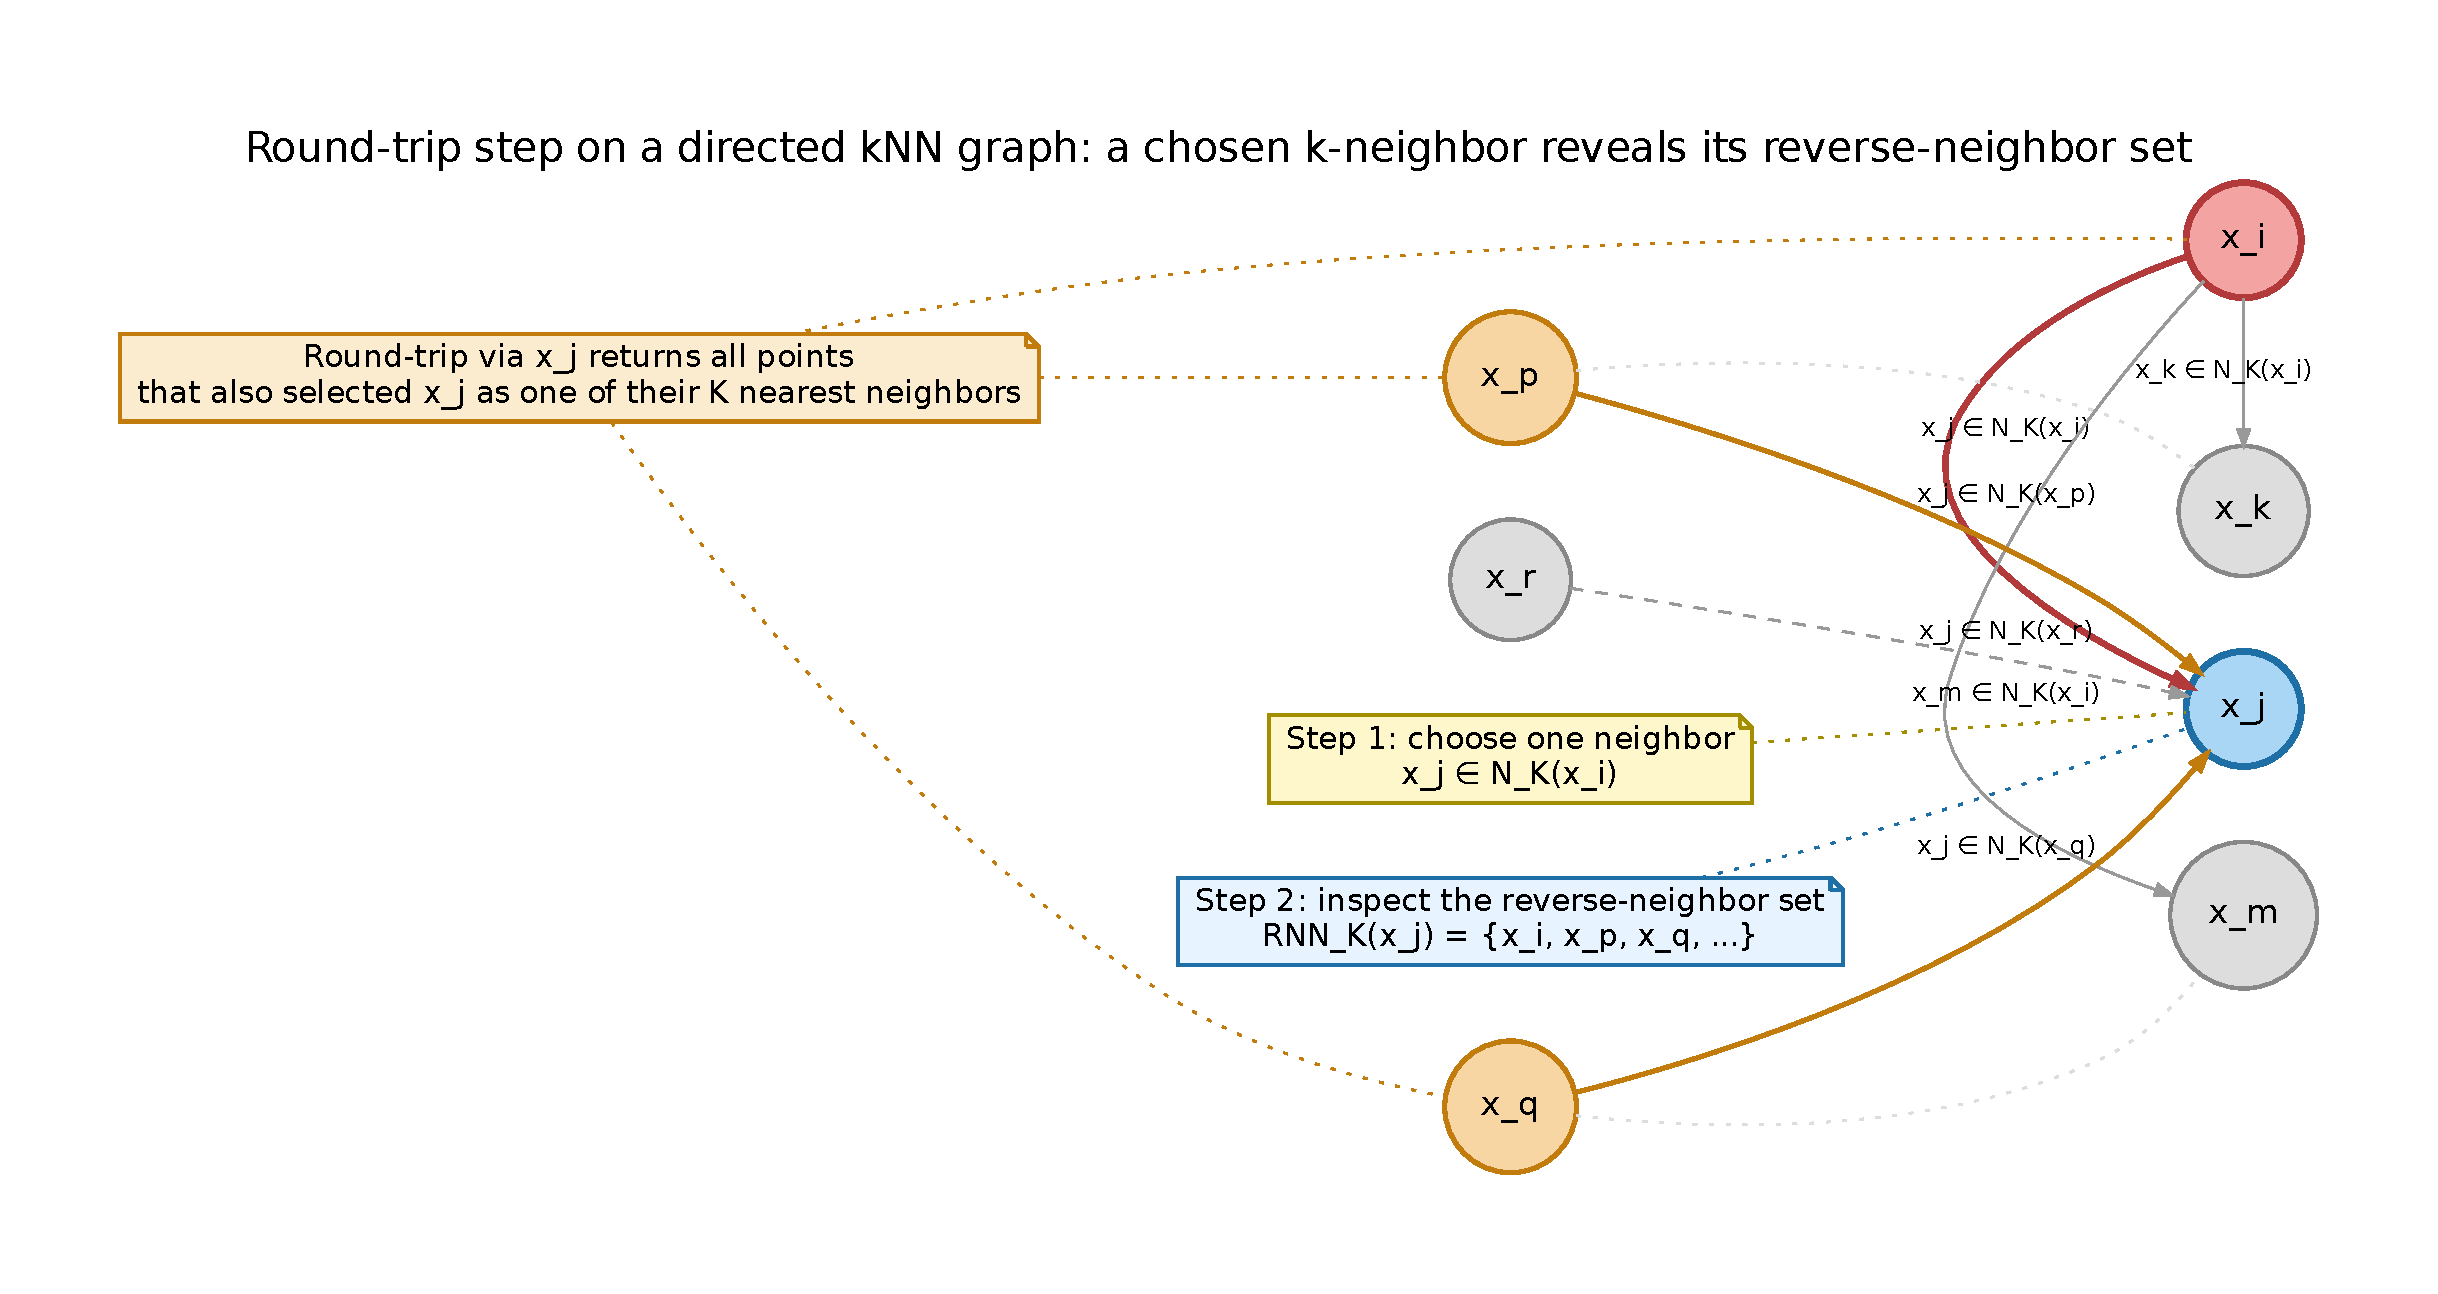
\includegraphics[width=0.88\linewidth]{figure1_roundtrip_reverse_neighbor.pdf}
\caption{Operational round-trip step on a directed KNN graph. A point $x_i$ selects $x_j$ as one of its $K$ nearest neighbors. The selected neighbor $x_j$ then reveals its reverse-neighbor set, i.e., all points that also selected $x_j$ as one of their $K$ nearest neighbors.}
\label{fig:roundtrip_reverse_neighbor}
\end{figure}

Figure~\ref{fig:roundtrip_reverse_neighbor} illustrates the elementary operation. The forward step is a standard KNN edge. The backward step is not a Euclidean displacement; it is a query to the reverse-neighbor set of the selected point. This is the local mechanism that links the 2018 KNN model to the older reflective composition $T^{-1}\circ T$.

\begin{definition}[Round-trip neighborhood]
Given $x_i\in X$, its one-step round-trip neighborhood is
\begin{equation}
\calR_K(x_i)=\bigcup_{x_j\in\calN_K^+(x_i)}\calN_K^-(x_j).
\label{eq:one_step_rt}
\end{equation}
\end{definition}

Equation~\eqref{eq:one_step_rt} can be restricted by selecting only one neighbor, for example the most popular neighbor in $\calN_K^+(x_i)$, or expanded by allowing all forward neighbors to contribute.

\section{Popularity-based leadership}\label{sec:leadership}

The 2018 formulation emphasized that a neighbor should be evaluated not only by its distance to the query point, but also by how many other points selected it as a nearest neighbor. This leads to a local leadership mechanism.

\begin{definition}[Local leader]
The popularity leader of $x_i$ at scale $K$ is
\begin{equation}
\ell_K(x_i)=\argmax_{x_j\in\calN_K^+(x_i)} \rdeg_K(x_j).
\label{eq:leader}
\end{equation}
\end{definition}

The leader $\ell_K(x_i)$ is one of the $K$ nearest neighbors of $x_i$, but it is chosen by reverse-neighbor popularity. Ties can be resolved by distance, by index order, or by retaining multiple leaders.

\begin{figure}[t]
\centering
\includegraphics[width=0.78\linewidth]{fig_2018_KNN_graph.pdf}
\caption{Example of a directed KNN graph from the 2018 prototype. Edges represent nearest-neighbor choices. The same graph supports reverse-neighbor counting and local leadership.}
\label{fig:KNN_graph_2018}
\end{figure}

\begin{figure}[t]
\centering
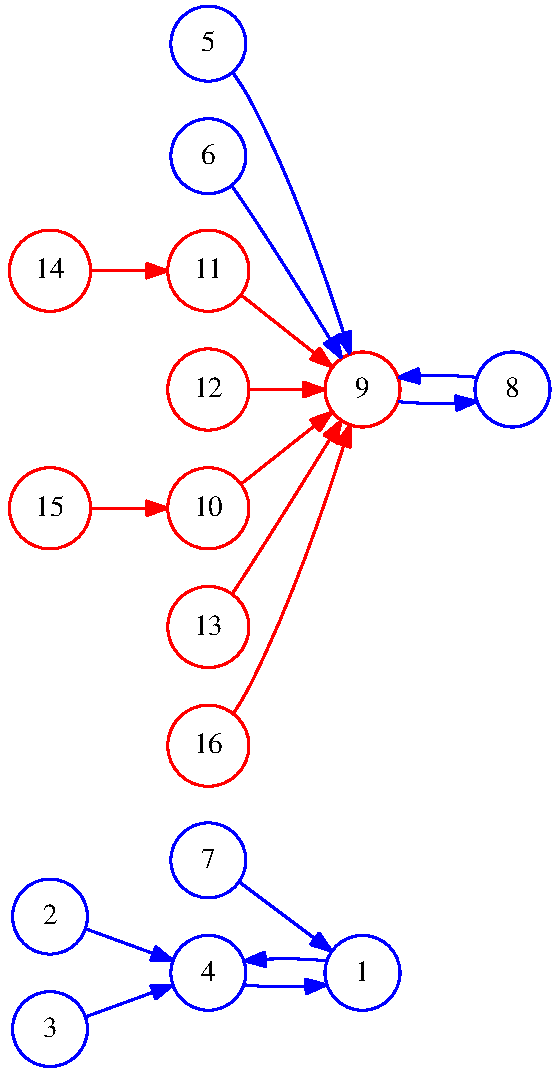
\includegraphics[width=0.78\linewidth]{fig_2018_leadership_graph.pdf}
\caption{Popularity-based leadership graph from the 2018 prototype. Each point points to a locally selected leader among its nearest neighbors according to reverse-neighbor popularity.}
\label{fig:leadership_2018}
\end{figure}

The leadership graph is a compressed directed structure obtained from the original KNN graph. It is not required that leadership alone define the final clustering, but it provides a useful mechanism for directing the round-trip expansion toward locally representative points.

\section{Recursive round-trip closure and saturation}\label{sec:closure}

The simplest closure version uses all forward neighbors:
\begin{equation}
C_K^0(x_i)=\{x_i\},
\end{equation}
\begin{equation}
C_K^{t+1}(x_i)=C_K^t(x_i)\cup
\bigcup_{x_q\in C_K^t(x_i)}\calR_K(x_q).
\label{eq:closure_all_neighbors}
\end{equation}
The process saturates when
\begin{equation}
C_K^{t+1}(x_i)=C_K^t(x_i).
\end{equation}
The saturated closure is denoted
\begin{equation}
C_K^\infty(x_i)=C_K^s(x_i),
\end{equation}
where $s$ is the first saturation time.

A leadership-driven variant is
\begin{equation}
C_K^{t+1}(x_i)=C_K^t(x_i)\cup
\bigcup_{x_q\in C_K^t(x_i)}\calN_K^-(\ell_K(x_q)).
\label{eq:closure_leadership}
\end{equation}
This version follows the reverse-neighbor set of the most popular local leader of each currently reached point.

\begin{algorithm}[t]
\caption{Leadership-driven round-trip closure for one point}
\label{alg:closure}
\begin{algorithmic}[1]
\Require directed KNN graph $\calG_K$, point $x_i$
\State $C \gets \{x_i\}$
\Repeat
    \State $C_{old}\gets C$
    \ForAll{$x_q\in C_{old}$}
        \State $y\gets \ell_K(x_q)$
        \State $C\gets C\cup\calN_K^-(y)$
    \EndFor
\Until{$C=C_{old}$}
\State \Return $C$
\end{algorithmic}
\end{algorithm}

The clustering step can then merge points whose saturated closures coincide or overlap above a prescribed threshold. In the current implementation, clusters are obtained from the induced layer output and then analyzed as partitions.

\section{Cluster layers and multiscale evolution}\label{sec:layers}

For a fixed $K$, the method yields a partition or cluster layer
\begin{equation}
\calP_K=\{C_1^{(K)},\ldots,C_{m_K}^{(K)}\}.
\end{equation}
By varying $K$ over a prescribed set of scales
\begin{equation}
K\in\{K_{\min},K_{\min}+1,\ldots,K_{\max}\},
\end{equation}
while keeping the basal parameter $K_0$ fixed, one obtains a multiscale sequence
\begin{equation}
\calP_{K_{\min}},\calP_{K_{\min}+1},\ldots,\calP_{K_{\max}}.
\end{equation}
In this notation, $K_0$ denotes the basal neighborhood scale from which the multiscale process is initiated, whereas $K$ denotes the current layer scale. Thus, the layer sequence should be interpreted as a controlled sweep over $K$ with $K_0$ kept fixed. This distinction is important in sparse-connectivity benchmarks, where an excessively large basal scale may prematurely merge regions connected by low-density bridges, while a smaller $K_0$ preserves the local structure long enough for bridge-like components to appear as separate clusters.
Increasing $K$ tends to increase graph connectivity. Therefore, small clusters from lower-$K$ layers are expected to be absorbed into larger clusters at higher $K$ values, although the exact behavior depends on the dataset and on the visibility or leadership rules.

The overlap between clusters in consecutive layers is
\begin{equation}
W_{ab}^{(K,K')}=|C_a^{(K)}\cap C_b^{(K')}|.
\label{eq:overlap_count}
\end{equation}
Useful normalizations include
\begin{equation}
F_{ab}^{(K,K')}=\frac{|C_a^{(K)}\cap C_b^{(K')}|}{|C_a^{(K)}|},
\label{eq:frac_from}
\end{equation}
and the Jaccard index
\begin{equation}
J_{ab}^{(K,K')}=\frac{|C_a^{(K)}\cap C_b^{(K')}|}{|C_a^{(K)}\cup C_b^{(K')}|}.
\label{eq:jaccard}
\end{equation}

\begin{figure}[t]
\centering
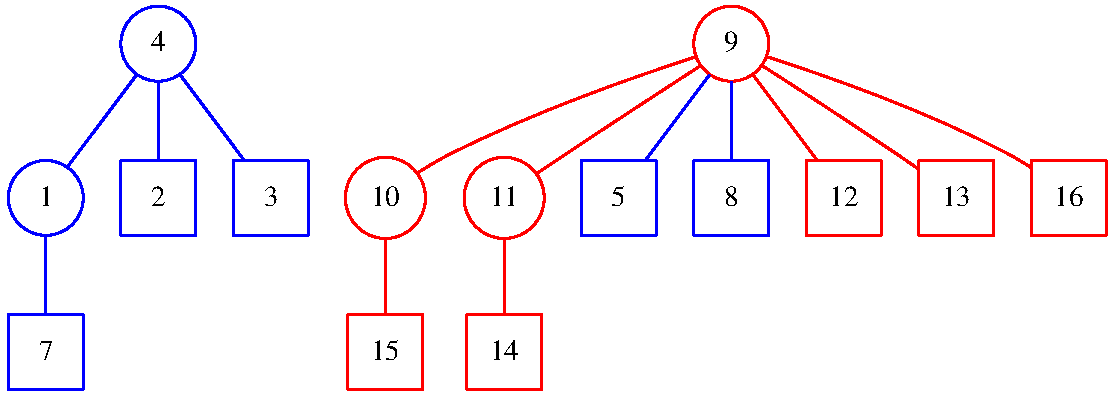
\includegraphics[width=0.75\linewidth]{fig_2018_cluster_tree.pdf}
\caption{Cluster-tree representation from the 2018 prototype. In the present formulation, this structure is reinterpreted as an ancestor of the $K$-layer transition graph, where clusters at smaller $K$ are progressively absorbed by larger-scale structures.}
\label{fig:cluster_tree_2018}
\end{figure}

\begin{figure}[t]
\centering
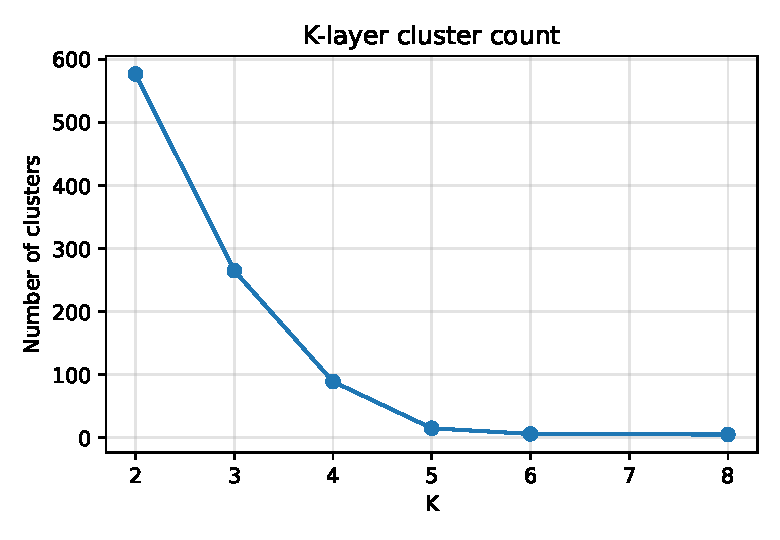
\includegraphics[width=0.75\linewidth]{fig_k_layer_cluster_count.pdf}
\caption{Preliminary $K$-layer evolution for a variable-density blobs dataset with $N=2000$ points. The number of clusters decreases as $K$ increases, indicating progressive absorption of microclusters into larger structures.}
\label{fig:k_layer_count}
\end{figure}

\section{Preliminary partition diagnostic}\label{sec:partition_diagnostic}

An important consistency check is whether each layer $\calP_K$ is a true partition of the dataset. For each $K$, this can be verified by comparing the sum of cluster cardinalities with the cardinality of the union of all cluster members:
\begin{equation}
\sum_{a=1}^{m_K}|C_a^{(K)}|=\left|\bigcup_{a=1}^{m_K}C_a^{(K)}\right|.
\label{eq:partition_check}
\end{equation}
When the equality in Eq.~\eqref{eq:partition_check} holds and the union contains all $N$ data points, the layer is not merely a cover of the dataset, but a proper partition:
\begin{equation}
\bigcup_{a=1}^{m_K} C_a^{(K)}=X,
\qquad
C_a^{(K)}\cap C_b^{(K)}=\varnothing
\quad\text{for }a\neq b.
\end{equation}
This property is important because the multiscale object produced by the algorithm is then a sequence of valid partitions, rather than a sequence of overlapping covers. Inter-layer overlap is still expected and informative, but intra-layer overlap would indicate an invalid layer representation.

If the left-hand side of Eq.~\eqref{eq:partition_check} is larger than the right-hand side, at least one point belongs to more than one cluster in the same layer.

For the preliminary variable-density blobs example, the diagnostic gave the results in Table~\ref{tab:partition_diagnostic}. Since all duplicate counts are zero, no internal overlap was detected within any analyzed layer.

\begin{table}[t]
\caption{Preliminary internal-overlap diagnostic for the variable-density blobs dataset. The equality between summed cluster sizes and number of unique points indicates that each layer is a valid partition.}\label{tab:partition_diagnostic}
\centering
\begin{tabular}{rrrrr}
\toprule
$K$ & number of clusters & summed size & unique points & duplicates\\
\midrule
2 & 577 & 2000 & 2000 & 0\\
3 & 265 & 2000 & 2000 & 0\\
4 & 89  & 2000 & 2000 & 0\\
5 & 15  & 2000 & 2000 & 0\\
6 & 6   & 2000 & 2000 & 0\\
8 & 5   & 2000 & 2000 & 0\\
\bottomrule
\end{tabular}
\end{table}

This diagnostic is different from inter-layer overlap. Inter-layer overlap is expected and informative; it describes how clusters from one scale are preserved, split, or absorbed at another scale.

\section{Scale, transmissivity, and confidence}\label{sec:scale}

The older relational notes contained an interpretation in terms of transmissivity and confidence. In the present graph setting, this can be reinterpreted as a scale-selection heuristic. Small $K$ values preserve local selectivity but may fragment the graph. Large $K$ values increase propagation but can dilute local evidence and eventually merge distinct structures.

Let $m$ denote the average number of forward links and $n$ the average reverse-neighbor count. The old balance condition can be written abstractly as
\begin{equation}
\tau\approx \frac{mn}{MN},\qquad \gamma\approx\frac{1}{mn},
\end{equation}
where $\tau$ measures propagation capacity and $\gamma$ measures confidence or selectivity. The balance $\tau=\gamma$ yields
\begin{equation}
(mn)^2=MN.
\end{equation}
In a standard directed KNN graph, $m\approx K$, while the mean reverse degree is also approximately $K$. Therefore, the average alone is not sufficient; the distribution of reverse degrees is more informative. Quantities such as
\begin{equation}
\operatorname{Var}(\rdeg_K),\qquad \max_i\rdeg_K(x_i),\qquad H(\rdeg_K)
\end{equation}
may help identify scales where local leadership is informative but not yet globally saturated.

\section{Experimental protocol}\label{sec:experimental_protocol}

The method should be evaluated on datasets that test distinct clustering difficulties:
\begin{itemize}
    \item Gaussian blobs with equal density;
    \item blobs with variable density;
    \item two moons;
    \item concentric circles;
    \item anisotropic clusters;
    \item uniform or Poisson-like point clouds;
    \item clusters connected by sparse bridges;
    \item orbital or astronomical time-series embeddings.
\end{itemize}

The bridge benchmark plays a complementary role to moons and circles. While moons and concentric circles test nonconvex separation, the bridge dataset tests robustness under sparse connecting structures. It evaluates whether the method collapses two dense regions into a single component merely because they are connected by a low-density chain of points, or whether the bridge is preserved as a meaningful intermediate structure. This benchmark is therefore useful for studying premature saturation, scale sensitivity, and the effect of the basal parameter $K_0$.

When labels are available, external validation should include the adjusted Rand index and normalized mutual information \citep{HubertArabie1985,VinhEppsBailey2010}. Internal criteria such as Davies--Bouldin, Calinski--Harabasz, and silhouette coefficients may also be reported \citep{DaviesBouldin1979,CalinskiHarabasz1974,Rousseeuw1987}, but should be interpreted carefully for nonconvex clusters. Baselines should include k-means, DBSCAN, HDBSCAN, SNN clustering, and mutual-KNN graph methods when available.

For each dataset and each $K$, the following quantities should be reported:
\begin{itemize}
    \item number of clusters $m_K$;
    \item cluster size distribution;
    \item saturation depth statistics;
    \item reverse-degree distribution;
    \item ARI and NMI when labels are known;
    \item internal validity indices;
    \item layer-transition overlaps $W_{ab}^{(K,K')}$ and normalized quantities $F_{ab}^{(K,K')}$ and $J_{ab}^{(K,K')}$.
\end{itemize}

\section{Discussion}\label{sec:discussion}

The method should be positioned carefully. It is not a first use of KNN graphs for clustering, nor a replacement for all density-based methods. Its distinctive aspect is the recursive use of forward KNN selection followed by reverse-neighbor retrieval, with popularity-based leadership and saturation. This places the method between shared-neighbor clustering, reverse-neighbor density reasoning, and graph-closure approaches.

The method is intentionally presented here as an algorithmic and topological construction, rather than as the minimization of an explicit objective function. Its definition does not reduce to a weighted voting rule, nor to the particular choice of a distance-based weight such as an inverse-square law. The central object is the dynamics induced on the directed KNN graph: forward-neighbor selection, reverse-neighbor retrieval, popularity, visibility, recursive expansion, and saturation. Whether this process admits an equivalent variational, probabilistic, or energy-based interpretation remains an interesting question for future work, but the absence of such a formulation is not a limitation of the graph operator itself.

Several points remain to be specified rigorously before a final submission:
\begin{enumerate}
    \item the exact closure rule used by the reference implementation;
    \item how ties in popularity leadership are handled;
    \item whether visibility constraints are mandatory or optional;
    \item how saturated closures are merged into final clusters;
    \item the computational complexity of the closure process;
    \item robustness to noise and outliers;
    \item behavior on homogeneous data, where saturation may correctly produce a single large component.
\end{enumerate}

\section{Conclusion}\label{sec:conclusion}

We presented a draft formulation of a clustering method based on round-trip closure in directed KNN graphs. The method combines a relational forward-backward idea, reverse-neighbor popularity, local leadership, recursive expansion, saturation, and multiscale $K$-layer analysis. The 2013 relational model provides the mathematical origin of the reflection operator, while the 2018 KNN prototype provides the algorithmic core based on reverse-neighbor discovery and popularity leadership. The modern formulation casts these ideas as a graph-based clustering variant suitable for systematic validation against established nearest-neighbor and density-based clustering methods.

\backmatter

\bmhead{Acknowledgements}

The authors thank collaborators who assisted in recovering and revising earlier implementations and manuscripts related to the round-trip KNN clustering approach.

\section*{Declarations}

\begin{itemize}
\item Funding: To be completed.
\item Conflict of interest/Competing interests: The authors declare that they have no competing interests. To be confirmed.
\item Ethics approval and consent to participate: Not applicable.
\item Consent for publication: Not applicable.
\item Data availability: Synthetic datasets and scripts will be made available in a public repository upon publication. To be completed.
\item Materials availability: Not applicable.
\item Code availability: The implementation will be made available in a public repository upon publication. To be completed.
\item Author contribution: To be completed.
\end{itemize}

% \bibliographystyle{plainnat}
% \bibliographystyle{sn-mathphys-num}
\bibliography{round_trip_KNN_refs}
\end{document}
